\section{Project showcase: an educational route from RTL to FPGA}

This section presents the project as a sequence of short, reproducible labs.
Each step produces something you can inspect: waveforms, traces, signatures, or
on-board memory state. Figure~\ref{fig:route-overview} gives the overall route
from editing the RTL to validating on the FPGA.

\begin{figure}[ht]
  \centering
  \fbox{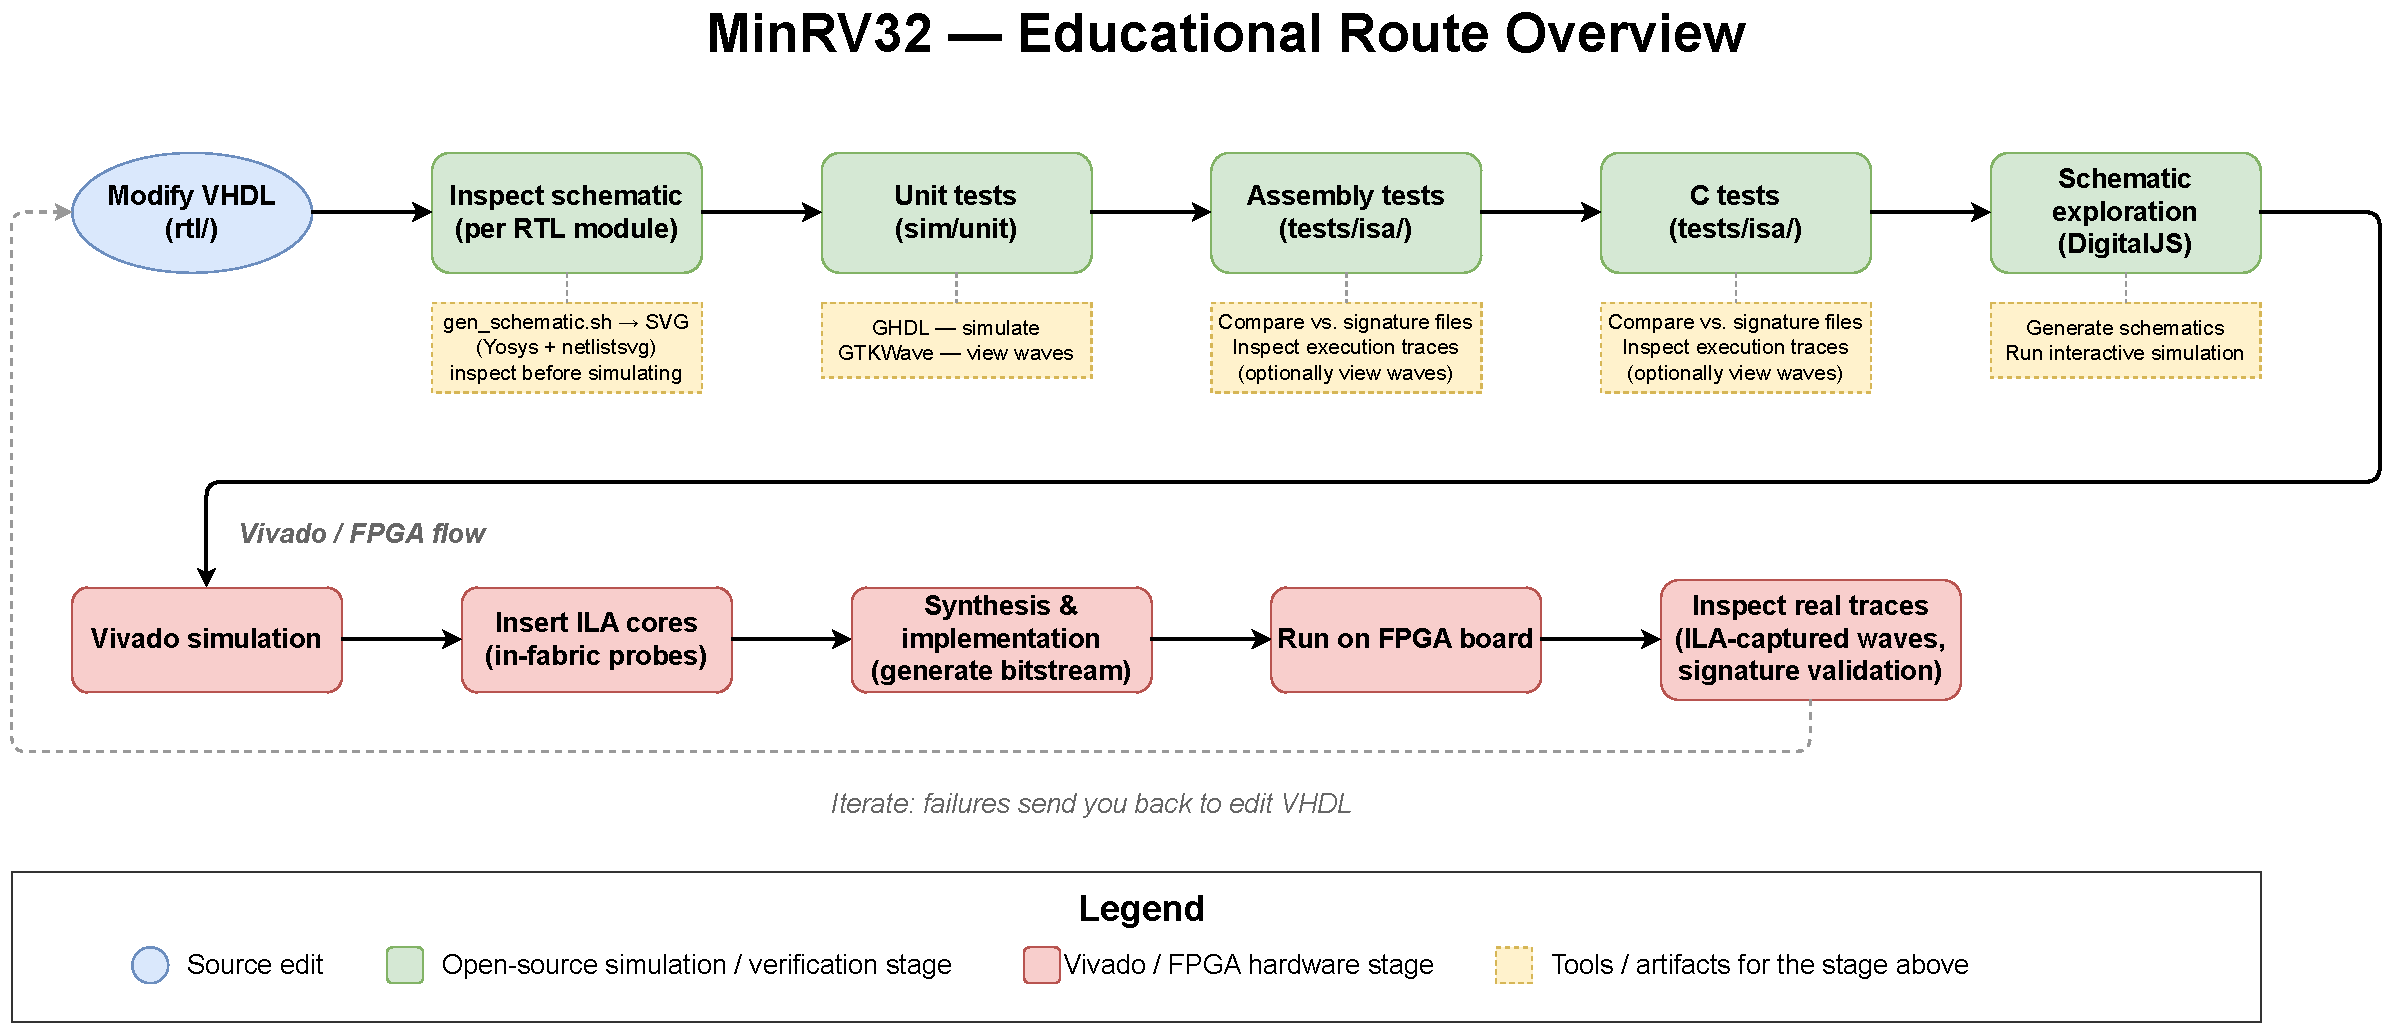
\includegraphics[width=0.97\linewidth]{educational_workflow.pdf}}
  \caption{Educational route overview. After editing the RTL, a module's
  schematic can be generated for inspection (Yosys + \texttt{netlistsvg}) before
  any simulation is run. After simulation, the design can be implemented and validated on the FPGA with an ILA capture.}
  \label{fig:route-overview}
\end{figure}

\subsection{Step 1: read/modify VHDL}

The RTL is modular (ALU, regfile, hazard unit, memory access helper, etc.), so a
change is usually localized to one small, readable entity.

\paragraph{Example VHDL: ALU combinational process (complete \texttt{case} statement)}
\lstinputlisting[style=minrv,language=VHDL,firstline=51,lastline=98]{../../rtl/alu.vhd}

\subsection{Step 2: inspect a module's schematic (before simulating)}

Before running any simulation, the structure of an edited module can be checked
visually. \texttt{scripts/gen\_schematic.sh} synthesizes an entity with Yosys
(via its GHDL front-end) and renders an SVG schematic with \texttt{netlistsvg},
so design mistakes are often caught just by looking at the elaborated logic.
\begin{lstlisting}[style=minrv]
./scripts/gen_schematic.sh --list           # list discoverable RTL entities
./scripts/gen_schematic.sh alu              # hierarchical schematic of one module
./scripts/gen_schematic.sh --flat 1 riscvpipe  # expand one level of hierarchy
\end{lstlisting}
The SVG lands under \texttt{build/schematics/<entity>.svg}
(Figure~\ref{fig:schematic-alu} shows the result for the \texttt{alu} entity).
The same tool underlies the microarchitecture block diagrams in this manual and
the DigitalJS export described in Step~6 (Section~\ref{sec:digitaljs}); see that
section for the prerequisite packages.

\begin{figure}[ht]
  \centering
  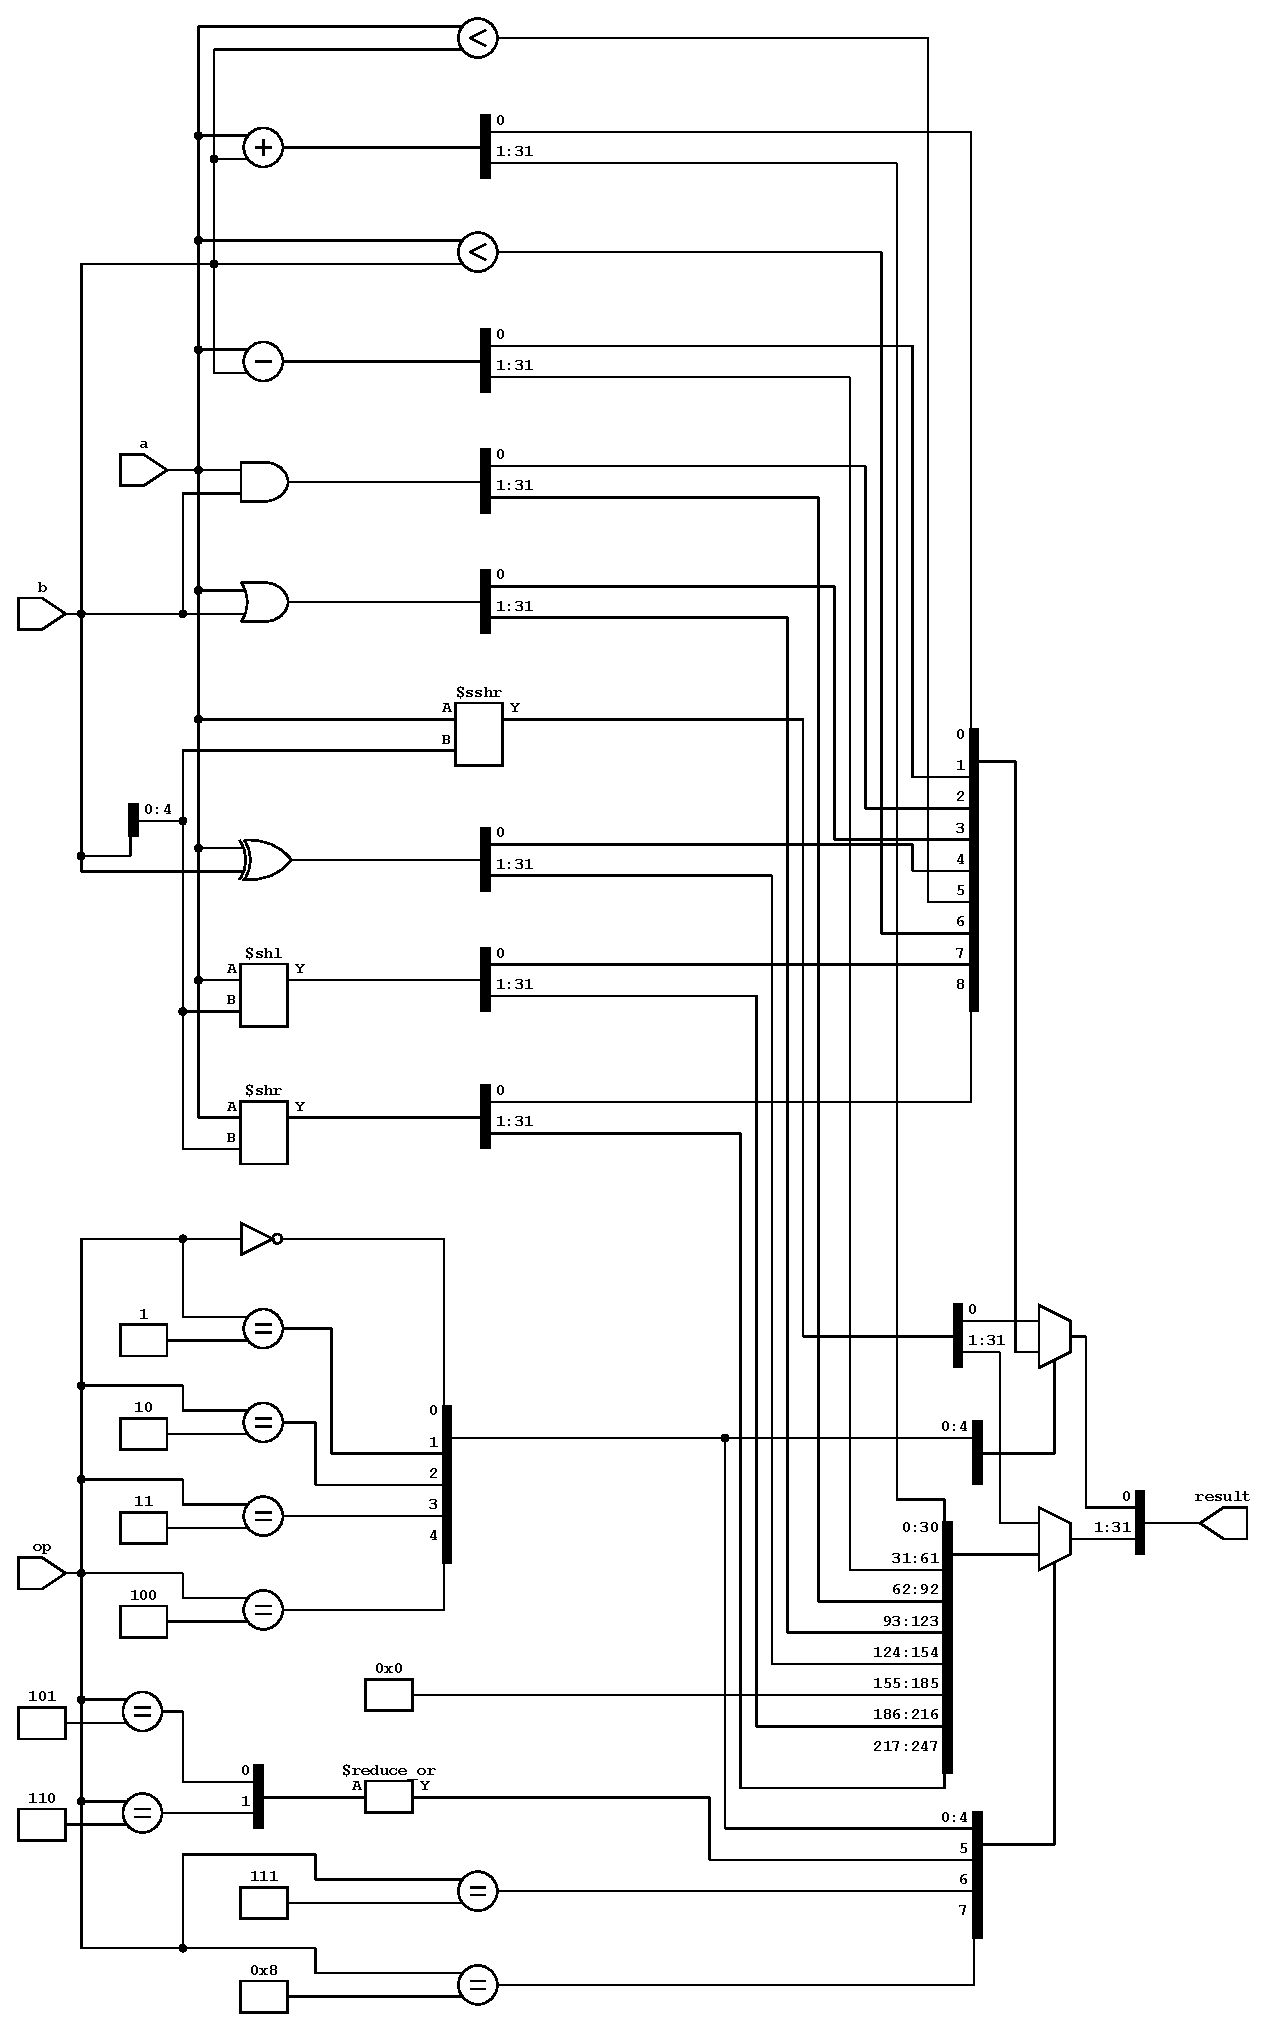
\includegraphics[height=0.82\textheight,keepaspectratio]{alu.pdf}
  \caption{Elaborated schematic of the \texttt{alu} entity rendered by
  \texttt{gen\_schematic.sh} (Yosys + \texttt{netlistsvg}). The \texttt{op}
  decoder (\texttt{\$eq} comparators, left of centre) selects, through the
  output multiplexers, one of the candidate results computed by the arithmetic,
  shift, and comparison operators. By default the script drops the
  multiplexers' don't-care default input for the unused \texttt{op} encodings
  (\texttt{opt\_expr -mux\_undef}), so no floating stubs clutter the diagram;
  pass \texttt{--keep-undef} to keep them.}
  \label{fig:schematic-alu}
\end{figure}

\subsection{Step 3: simulate modules with unit testbenches}

For component bring-up, the repository includes small self-checking unit
testbenches under \texttt{sim/unit/}.

\paragraph{Example unit testbench: checking the ALU (complete architecture body)}
\lstinputlisting[style=minrv,language=VHDL,firstline=89,lastline=116]{../../sim/unit/tb_alu.vhd}

\paragraph{Run + dump waves}
\begin{lstlisting}[style=minrv]
./scripts/run_unit_tb.sh --fst alu
./scripts/view_wave.sh build/waves/tb_alu.fst
\end{lstlisting}
GTKWave then shows the unit-test waveform (Figure~\ref{fig:wave-tb-alu}).

\begin{figure}[ht]
  \centering
  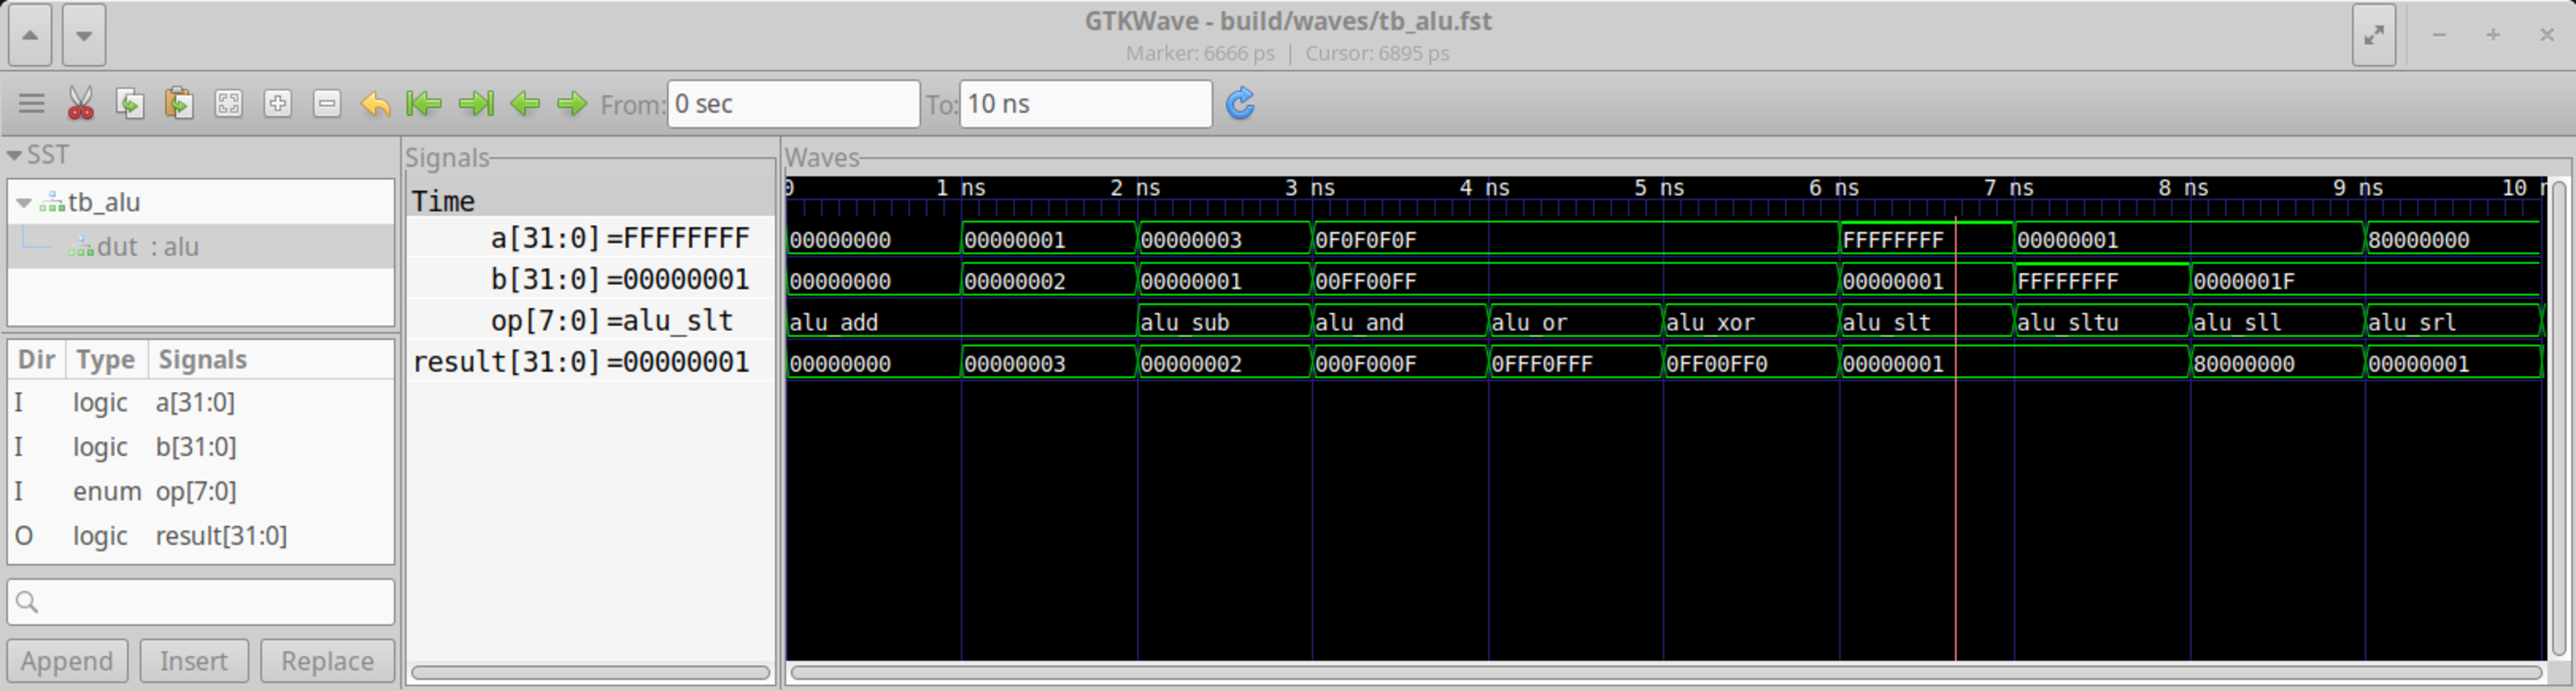
\includegraphics[scale=0.29]{gtkwave-tb_alu.pdf}
  \caption{Unit-test waveform.}
  \label{fig:wave-tb-alu}
\end{figure}

\subsection{Step 4: run assembly tests (correctness via signature + optional traces/waves)}

Integration tests live under \texttt{tests/isa/}. Each test writes a signature
window into DMEM at \texttt{0x20000100}. The expected values are stored in
\texttt{tests/isa/<name>.sig}, and the testbench compares observed vs expected.

\paragraph{Example assembly test: write 6 signature words}
\lstinputlisting[style=minrv,firstline=1,lastline=32]{../../tests/isa/addi_only.S}

\paragraph{Run + view trace and waves}
\begin{lstlisting}[style=minrv]
./scripts/run_test.sh --trace addi_only
./scripts/run_test.sh --fst addi_only
./scripts/view_wave.sh build/waves/addi_only.fst
\end{lstlisting}

\paragraph{Per-instruction trace: decoded ASM + stage control sample output}
\lstinputlisting[style=minrv,firstline=22,lastline=49]{../common/sample_output/addi_only_trace.txt}

\subsection{Step 5: run freestanding C tests (same signature mechanism)}

Freestanding C tests follow the same rule: compute deterministic values, then
store them into the signature window at \texttt{0x20000100}.

\paragraph{Example C: tests/isa/factorial.c}
\lstinputlisting[style=minrv,language=C,firstline=1,lastline=31]{../../tests/isa/factorial.c}

\paragraph{Run + view trace and waves}
\begin{lstlisting}[style=minrv]
./scripts/run_test.sh --trace factorial
./scripts/run_test.sh --fst factorial
./scripts/view_wave.sh build/waves/factorial.fst
\end{lstlisting}

\paragraph{Example test output snippet without trace}
\lstinputlisting[style=minrv,firstline=9,lastline=20]{../common/sample_output/factorial.txt}

The resulting execution waveform for computing $6!$ is shown in
Figure~\ref{fig:wave-factorial}.

\begin{figure}[ht]
  \centering
  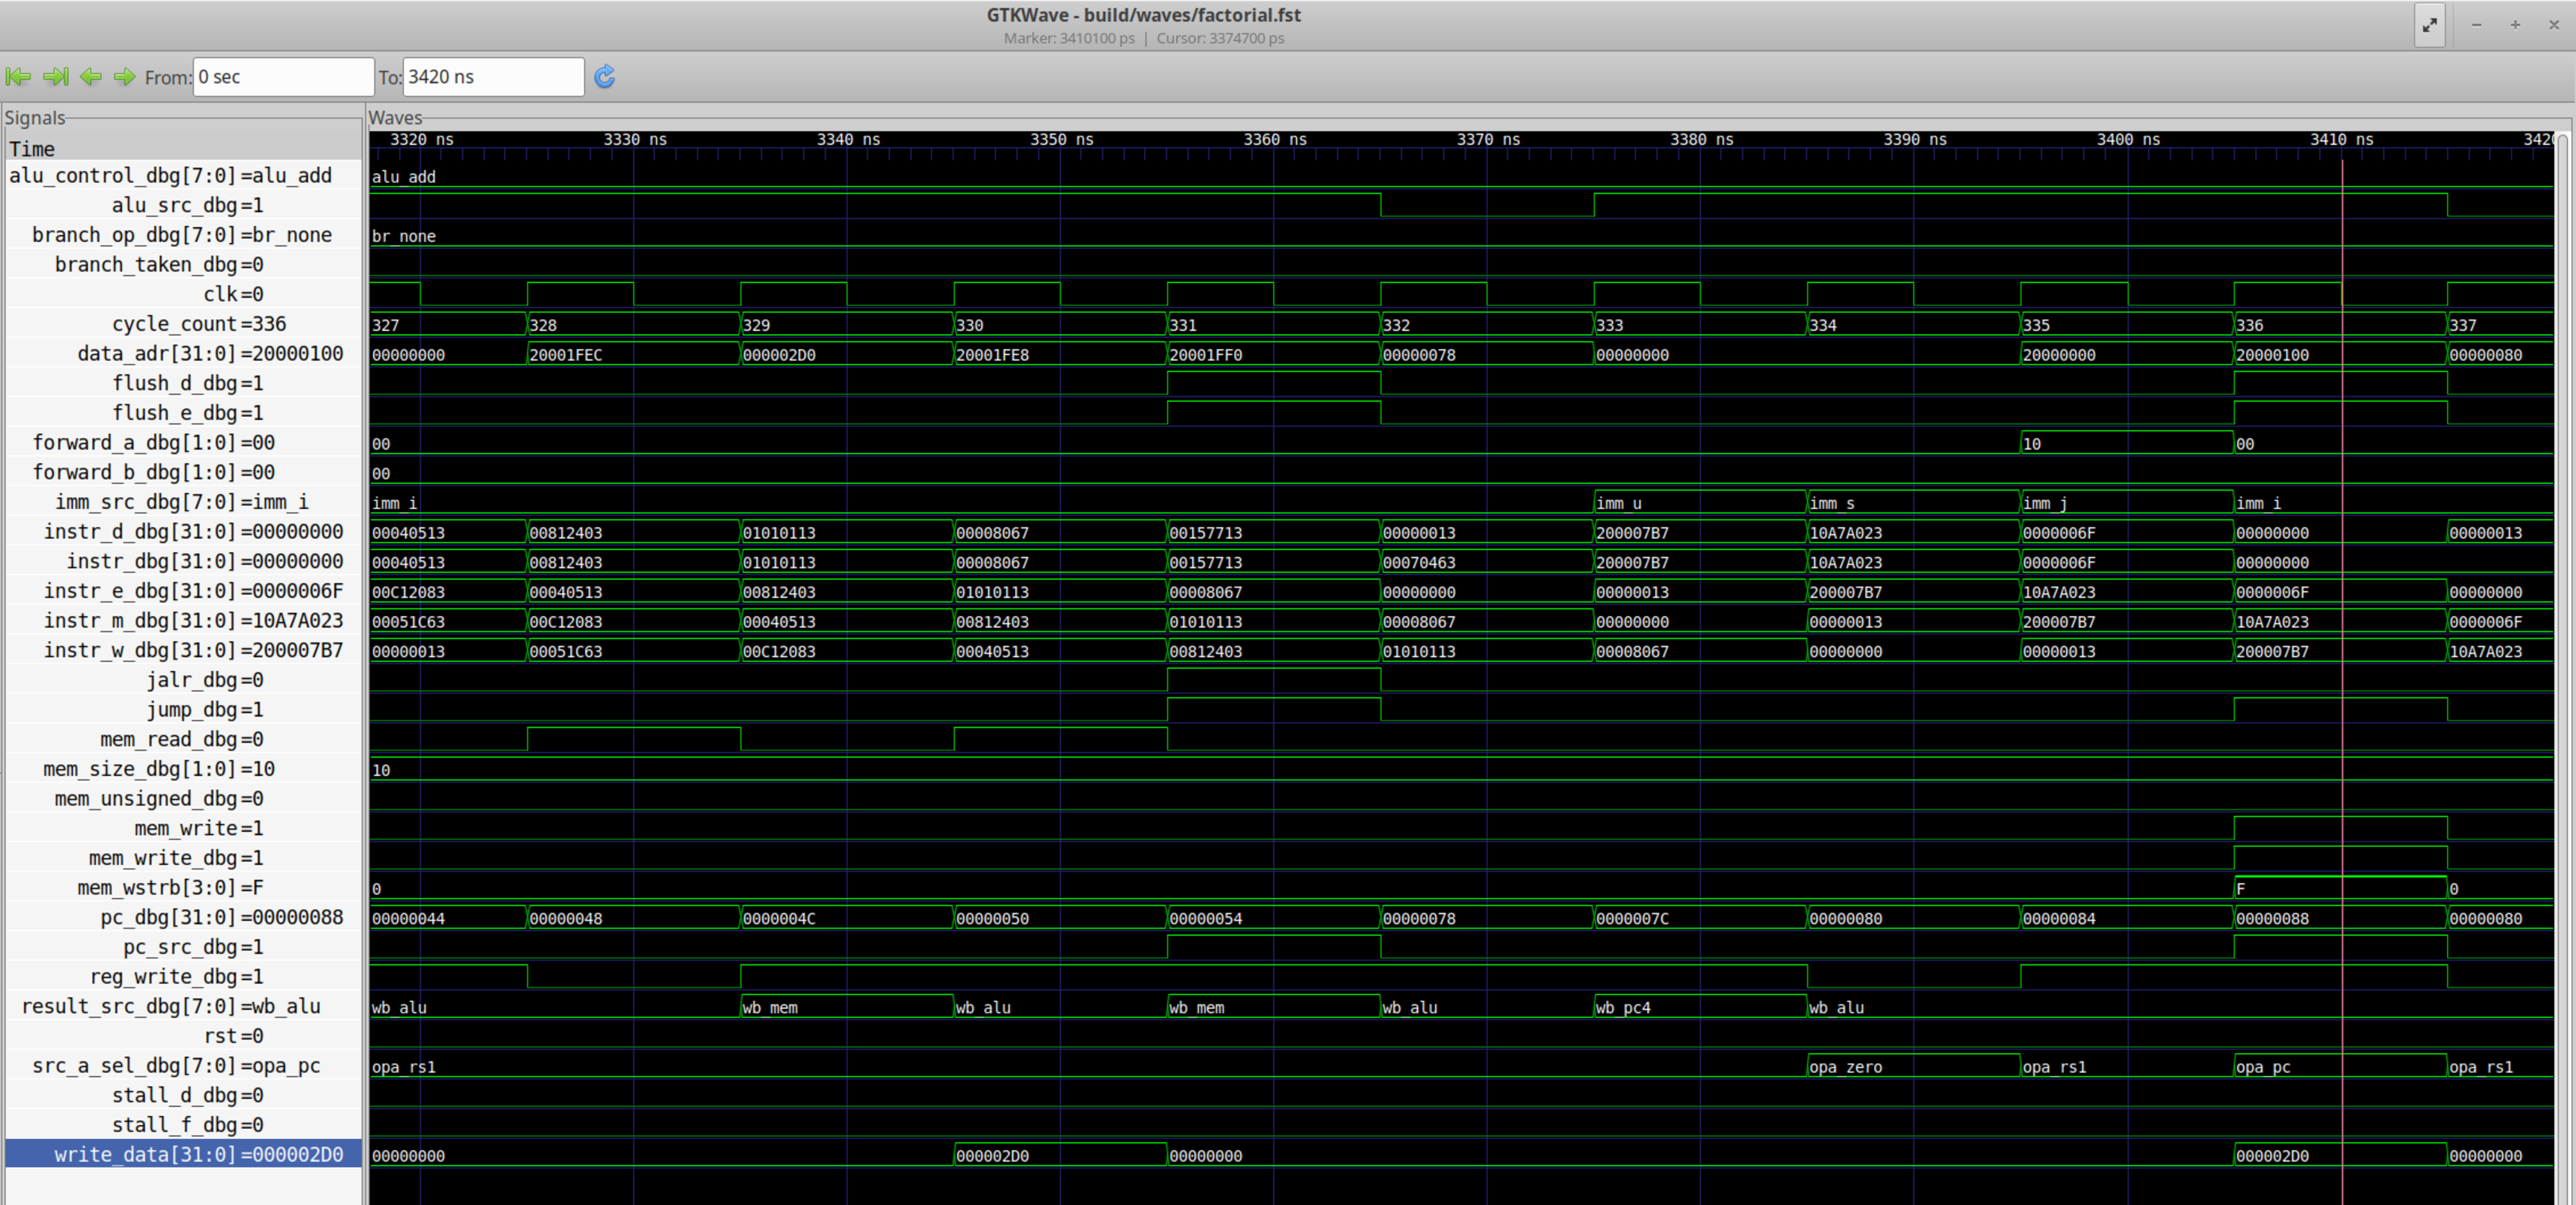
\includegraphics[scale=0.2]{gtkwave-factorial.pdf}
  \caption{Factorial C program execution waveform for calculating 6!}
  \label{fig:wave-factorial}
\end{figure}

\subsection{Step 6: explore the design interactively in DigitalJS}

The same netlist that produces the static schematics of Step~2 can be exported
to DigitalJS for interactive, in-browser simulation: drive inputs by clicking
and watch values propagate through the gates. With real firmware pre-loaded it
even single-steps the whole pipeline. This is a visual complement to GTKWave
(for leaf modules) and to the full-core tests (for the whole pipeline); it is
not signature-checked, so it does not replace the testbench pass/fail. See
Section~\ref{sec:digitaljs} for the commands and the firmware-loaded export.
Although the simulation is not signature-checked, it is a powerful tool
for visually confirming the design's behaviour on the FPGA, where visibility
is limited to the ILA capture points. Additionally, the signature values written
in the DMEM, usually at the end of the executed program, can be manually
verified against the expected values in the corresponding \texttt{.sig} file. 

\subsection{Step 7: implement on FPGA and validate with an ILA capture}

After simulation passes, Vivado can synthesize and implement the same RTL. On
hardware, you validate results with an Integrated Logic Analyzer (ILA)
triggered on stores into the signature window -- the same \texttt{.sig} words
that simulation already checks (Figure~\ref{fig:ila-full_core}).

\paragraph{Content of the tests/isa/full\_core.sig file}
\lstinputlisting[style=minrv,firstline=1,lastline=10]{../../tests/isa/full_core.sig}

\begin{figure}[ht]
  \centering
  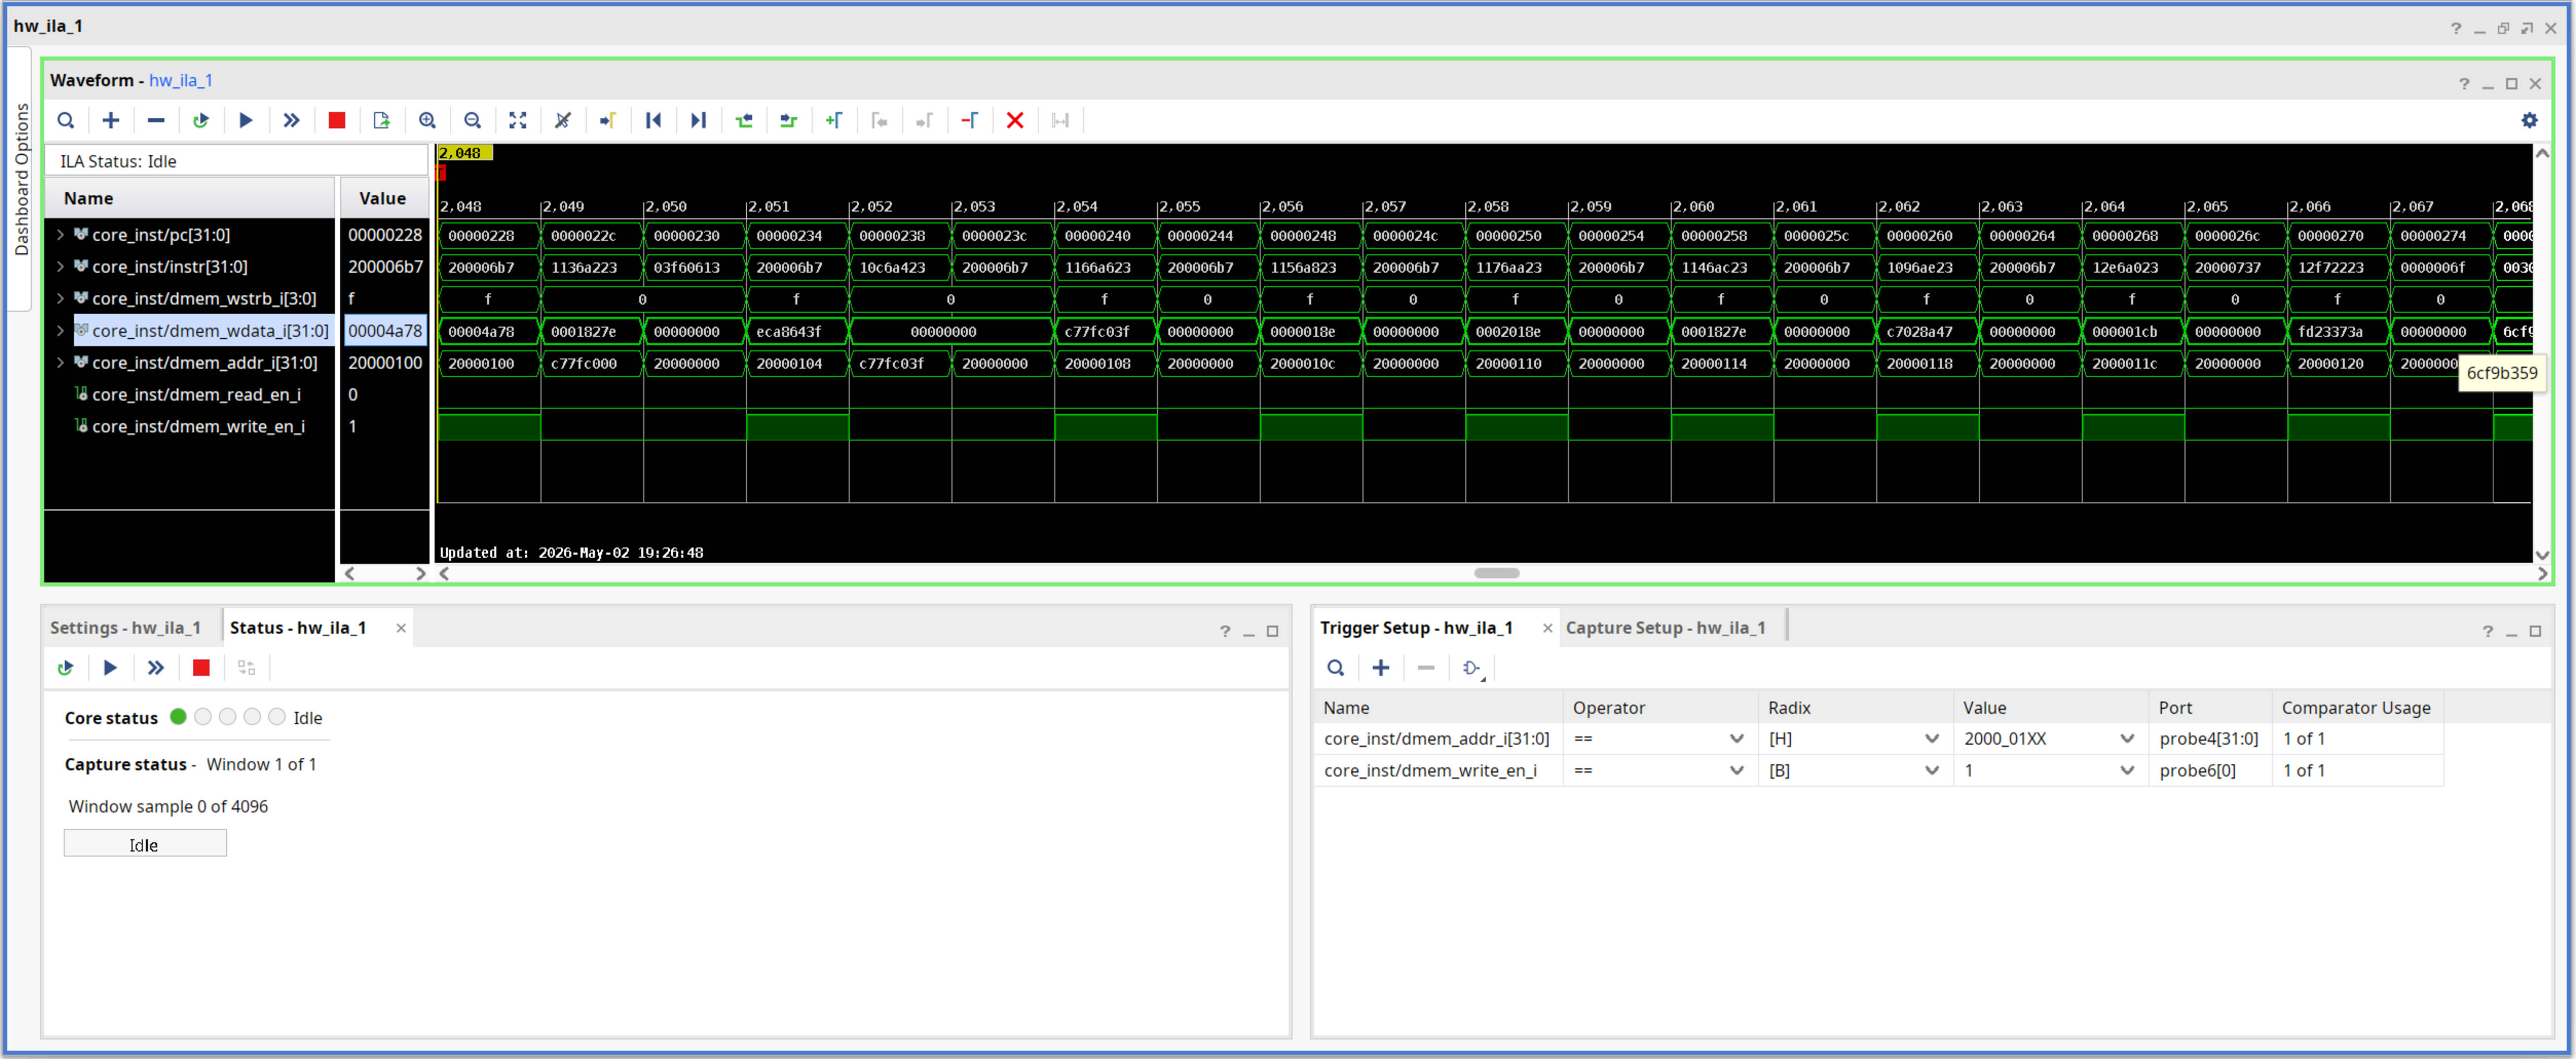
\includegraphics[scale=0.18]{ila-full_core.pdf}
  \caption{Hardware Manager + ILA waveform capturing signature stores of the full\_core.c program running on MinRV32 on the FPGA.}
  \label{fig:ila-full_core}
\end{figure}
